\documentclass[10pt]{article}
\usepackage[latin1]{inputenc}
\usepackage[english]{babel}
\usepackage{fancyvrb}
\usepackage[a4paper,margin=2cm]{geometry}
\usepackage{titlesec}
%\usepackage{macrosens}
\usepackage{comment}
\usepackage{mathpazo}
\usepackage{ dsfont }
\usepackage{amsmath}
\usepackage{hyperref}
\usepackage{color}
\usepackage{graphicx}


%\setlength{\parindent}{0pt}
\setlength{\parskip}{1ex}

%\titleformat{ command }[ shape ]{ format }{ label }{ sep }{ before }[ after ]
%\titleformat{\section}{\large\bfseries}{Exercise \thesection.}{1ex}{}
%\titlespacing{\subsection}{0pt}{*2}{*1}

\renewcommand{\thesubsection}{\arabic{subsection}}

\titleformat{\subsection}[runin]{\normalsize\bfseries}{Q\thesubsection.}{1ex}{}
\titlespacing{\subsection}{0pt}{*2}{*1}

\specialcomment{correction}
{\begin{quote}
    \begin{em}
      \begin{tabular}{|p{\linewidth}|}\hline
      }{
        \\\hline
      \end{tabular}
    \end{em}
  \end{quote}
}

\newcommand{\smallcorr}[1]{\hfill\emph{\begin{tabular}[c]{|l|}\hline #1\\\hline\end{tabular}}}
% 2 lines below to comment to get the correction
\renewcommand{\smallcorr}[1]{}
\excludecomment{correction}

\begin{document}

\pagestyle{empty}

\noindent
\textbf{IST Austria} \hfill %\textbf{Polytech Grenoble} \\
\textbf{Numerical Algorithms} \hfill \textbf{Spring 2017}





%\lstset{
%  language=Algo,
%  basicstyle=\sffamily,
%  columns=fullflexible,
%  mathescape
%}

\begin{center}
{\large\textbf{Homework 3: Optimization}}\\
Due Wednesday,April 3.
\end{center}

\noindent\makebox[\linewidth]{\rule{\linewidth}{0.6pt}}
 
\section*{Instructions}

\begin{itemize}
\item The assignments must be dropped off in the T.A. mail box: Office Building West, 2nd floor, left of the stairs, top-left box, or sent to me by email. The deadline is April 3 at midnight.
\item The assignments may be handwritten or typed. You can code in any programming language. The code itself will not be reviewed. 
\item The textbook is \emph{Numerical Algorithms} from Justin Solomon.\\ \url{https://people.csail.mit.edu/jsolomon/share/book/numerical_book.pdf}.  
\end{itemize}



\noindent\makebox[\linewidth]{\rule{\linewidth}{0.6pt}}

\section*{Exercise 1: Trapezoidal method \normalsize \textnormal(25 points)}

Let's $\vec{y}: \mathds{R} \rightarrow \mathds{R}^n$ be a function satisfying the ODE:
$$\vec{y}'= F(\vec{y}), \vec{y}(0) = \vec{y}_0.$$
We define $\vec{y}_k = \vec{y}(t_k) = \vec{y}(kh)$ with $h$ a time step $> 0$.

\subsection{} Use the trapezoidal quadrature rule to show that:
$$\vec{y}_{k+1} \approx \vec{y}_k + h\frac{F(\vec{y}_{k+1}) + F(\vec{y}_k)}{2}$$

This ODE integrator is called the \emph{trapezoidal method}.

\subsection{} What can you say about the accuracy of this method ?

\subsection{} Using the model equation $y' = ay$, with $a < 0$, analyse the stability of the method.

\subsection{} Despite its higher order of accuracy with maintained stability, the trapezoid method has some drawbacks that make it less popular than backward Euler for large time steps. Let's consider the ratio $R = \frac{y_{k+1}}{y_k}$. What is the value of $R$ when the time step $h \to \infty$. What does it say about the behaviour of the solution obtained with the trapezoidal method.

\subsection{} The trapezoidal method is an implicit integrator. Use an Euler step to approcimate $F(\vec{y}_{k+1})$ and derive an explicit method. This method is called Heun's method. Analyse the accuracy and stability of this method.

\section*{Exercise 2: Verlet algorithm \normalsize \textnormal(5 points) \textit{(from the textbook)}}

\subsection{} Suppose we wish to approximate solutions to $\vec{y}'' = F(\vec{y})$. Add together Taylor expansions for $\vec{y}(t + h)$ and $\vec{y}(t - h)$ to derive the \emph{Verlet algorithm} for predicting $\vec{y}_{k+1}$ from $\vec{y}_k$  and $\vec{y}_{k-1}$ , which induces $O(h^4)$ integration error in a single time step.

15.4 p342\\

\section*{Exercise 3: Pendulum algorithm \normalsize \textnormal(20 points) \textit{(from the textbook)}}

The swing angle $\theta$ of a pendulum under gravity satisfies the following ODE:
$$\theta'' = -\sin \theta,$$
where $|\theta(0)| < \pi$ and $\theta'(0) = 0$.

\subsection{} Suppose $\theta(t)$ solves the ODE. Show that the following value (representing the energy of the system) is constant as a function of $t$:
$$E(t) = \frac{1}{2}(\theta')^2 - \cos \theta.$$

\subsection{} Many ODE integrators drift away from the desired output as time progresses over larger periods. For instance, forward Euler can add energy to a system by overshooting, while backward Euler tends to damp out motion and remove energy. In many computer graphics applications, quality long-term behavior can be prioritized, since large-scale issues cause visual artifacts. The class of symplectic integrators is designed to avoid this issue.

Denote $\omega = \theta'$. The symplectic Euler scheme makes a series of estimates $\theta_ 0$, $\theta_ 1$, $\theta_ 2$, $\theta_ 3$, $\hdots$ and $\omega_0$, $\omega_1$, $\omega_2$, $\omega_3$, $hdots$ at time $t = 0$, $h$, $2h$, $3h$, $\hdots$ using the following iteration:
$$\theta_{k+1} = \theta_k + h\omega_k$$
$$\omega_{k+1} = \omega_k - h \sin \theta_{k+1}.$$
Define
$$E_k = \frac{1}{2}\omega^2 - \cos \theta_k.$$
Show that $E_{k+1} = E_k + O(h^2)$.

\subsection{} \label{q} Suppose we make the small-angle approximation $\sin \theta \approx \theta$ and decide to solve the linear ODE $\theta'' = -\theta$ instead. Now, symplectic Euler takes the following form:
$$\theta_{k+1} = \theta_k + h\omega_k$$
$$\omega_{k+1} = \omega_k - h\theta_{k+1}.$$
Write a $2 \times 2$ matrix $A$ such that:
$$
\left(\begin{matrix}
  \theta_{k+1} \\
  \omega_{k+1}
  \end{matrix} \right)
=
A
  \left(\begin{matrix}
     \theta_k \\
  \omega_k
  \end{matrix} \right)
  .$$

\subsection{} If we define $E_k = \omega^2 + h\omega_k\theta_k + \theta^2$ , show that $E_{k+1} = E_k$ in the iteration from Q\ref{q}. In other words, $E_k$ is constant from time step to time step.
  
15.7 p343
 
\section*{Exercise 4: Springs \normalsize \textnormal(50 points)}


\begin{wrapfigure}{l}{0.2\textwidth}
  \centering
  \vspace{-0.5cm}
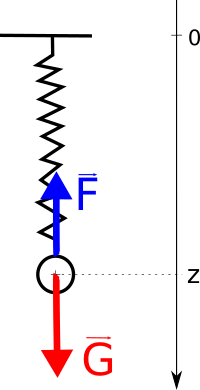
\includegraphics[width=0.19\textwidth]{spring.png}
\vspace{-1cm}
\end{wrapfigure}

We consider that a spring of stiffness $k$, of length at rest $l_0$ and current length $l$ attached to a small mass $m$ applies a force $\vec{F} = k\frac{l - l_0}{l_0} \vec{d}$ where $\vec{d}$ is the normalized direction of the spring.

\subsection{1D spring} Let's consider the case of a vertical spring attached at one side to a fixed point at the other to the mass $m$. The position of the fixed point is $z = 0$ and the position of the mass at time $t$ is $z = z(t)$. Let's ignore for know the gravity. Using Newton's second law and forward Euler, write a programme computing the position of the mass through time according taking in entry the length at rest $l_0$ and stiffness $k$ of the spring, the value of the mass $m$, the inital position $z_0$ and $v_0$ of the mass, and a time step $h$.

In what range should one choose $h$ for the method to be stable ?
Plot $z(t)$ for $k = $, $m = $, $l_0 = 10cm$, $z_0 = 12cm$ and $v_0$ for a stable time step and an unstable one.

Modify now the method to use backward Euler. Plot $z(t)$ for the same time steps used at the previous question.

\subsection{Gravity} Let's consider now that the gravity also applies a force $\vec{G} = - m g \vec{z}$ where $\vec{z}$ is the up direction and $g = 9.81m.s^{-2}$. Plot the position $z(t)$ and see at which lenght of the spring the system reach a stable position. Is this corresponding to the theoretical stable position ?


\end{document}
